\section{Baseline MLP}
\begin{itemize}
    \item Final training accuracy: \textbf{99.79 \%}
    \item Final validation accuracy: \textbf{97.74 \%}
    \item Number of parameters:  \textbf{535,818}
\end{itemize}

\begin{figure}[h]
    \centering
    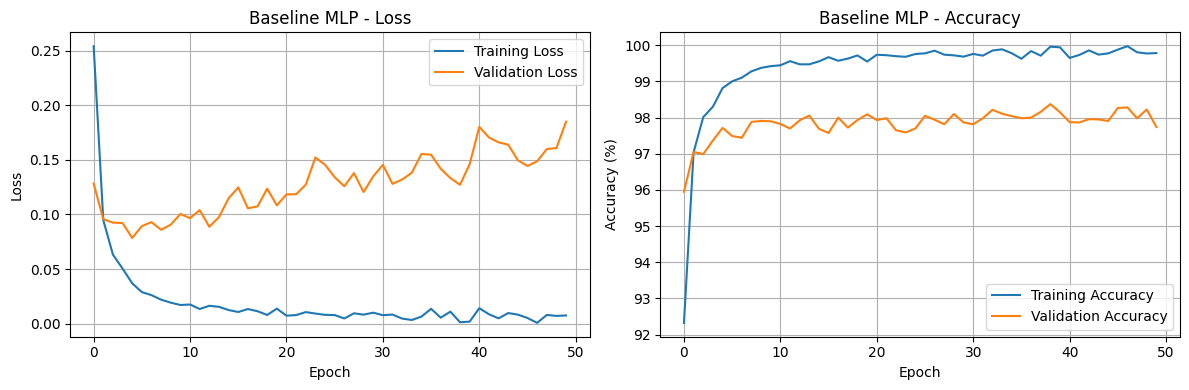
\includegraphics[width=0.5\linewidth]{section1/baselineMLP.png}
    \caption{Caption}
    \label{fig:placeholder}
\end{figure}

\subsection{Is the model overfitting?}
Yes, the model is overfitting. The training loss approaches zero while validation loss increases after epoch 10, and there's a 2\% gap between training (99.79\%) and validation (97.74\%) accuracy, indicating the model memorizes training data rather than generalizing.

\subsection{At approximately which epoch does overfitting begin?}
Overfitting begins around epoch 10-15, observable when validation loss stops improving and starts increasing while training loss continues to decrease.

\subsection{Conclusion}
It means that the model is too powerful for this task. It has 535,818 parameters and learns the training data too well which including noise and specific details that don't generalize.

